\section{Estimator bias}

\mode<presentation>{
\begin{frame} 
    \begin{center} \huge
        \secname
    \end{center}
    \begin{center}
        How good is our estimation method?
    \end{center}
	
\end{frame}
}

%%%%%%%%%%%%%%%%%%%%%%%%%%%%%%%%%%%%%%%%%%%%%%%%%%%%%%%%%%%%%%%
\begin{frame}{Parameters are also random variables}

Assume $\vec x^{(\alpha)} \sim P(\vec x; \vec w^*)$, i.e. $\vec x^{(\alpha)}$ is a random vector, and $\vec w^*$ the true parameters of a the data generating distribution.\\

\svspace{3mm}

Our estimator yields an estimate $\widehat{\vec w} = f(\vec x^{(1)}, \ldots,\vec x^{(p)})$ $\Rightarrow$ $\widehat{\vec w}$ is also a random variable\\

\svspace{3mm}

Example: MLE $\widehat{\vec w}_{\text{ML}} = \argmax_{\vec w} \widehat P(\vec x^{(1)}, \ldots,\vec x^{(p)}; \vec w)$\\

\pause 

\question{Where does the randomness come from?}

\pause

-Different data sets with $p$ samples from the same distribution lead to different estimates $\widehat{\vec w}$

\pause

\svspace{3mm}

$\Rightarrow$ The random vector $\widehat{\vec w}$ has moments, e.g. mean $\langle \widehat{\vec w} \rangle_{P(\vec x^{(1)}, \ldots,\vec x^{(p)}; \vec w^*)}$

\end{frame}

\subsection{Bias of an estimator}

\begin{frame}{\subsecname}

bias $\vec b := \langle \widehat{\vec w} \rangle - \vec w^*$

If $b=0$, then our estimator is \textbf{un}biased

\underline{Interpretation}: Draw multiple data sets of size $p$, then the estimated parameters will surround the true vector $\vec w^*$.

\begin{center}
	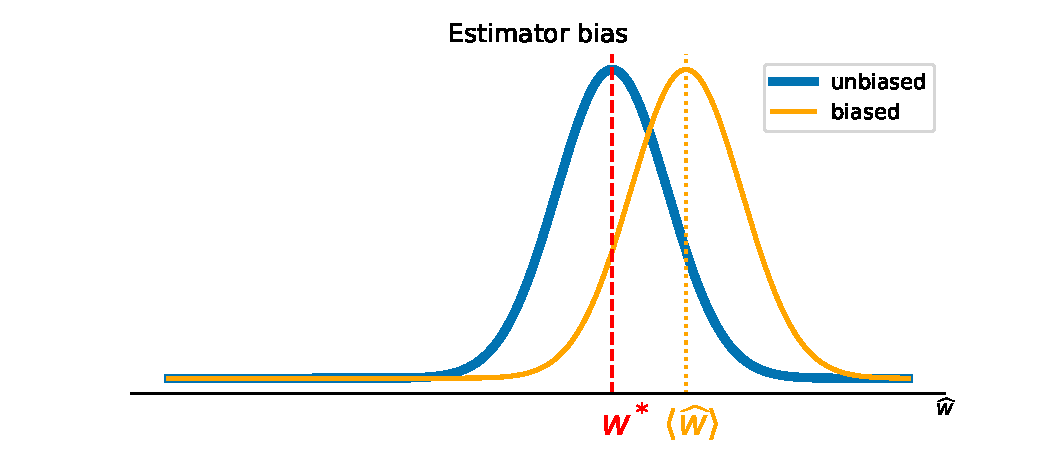
\includegraphics[width=0.6\textwidth]{img/bias.pdf}
	\notesonly{\captionof{figure}{Estimator bias}}
\end{center}


\end{frame}

\subsection{Variance also plays a role}

\begin{frame}{\subsecname}

\begin{center}
	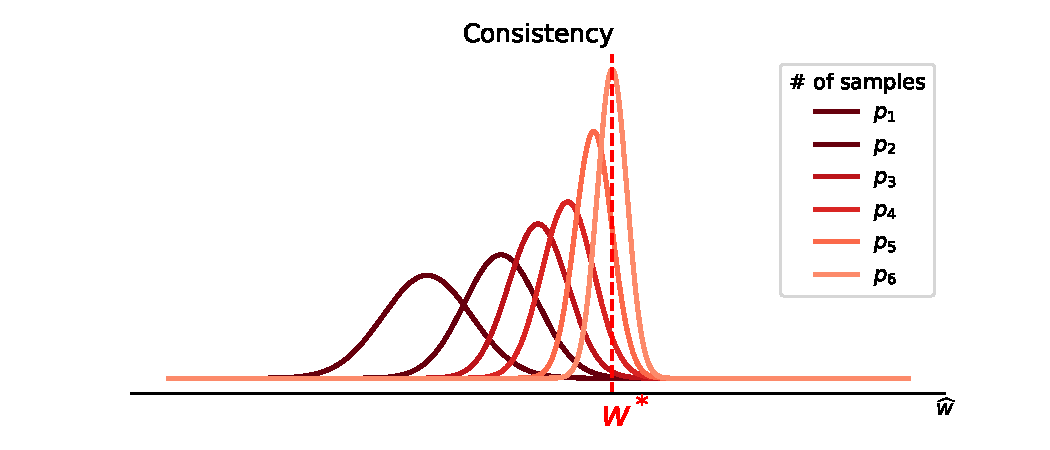
\includegraphics[width=0.6\textwidth]{img/consistency.pdf}
	\notesonly{\captionof{figure}{A consistent estimator converges in probability to the true value when given more data.}}
\end{center}

\end{frame}
